%% LyX 2.3.7 created this file.  For more info, see http://www.lyx.org/.
%% Do not edit unless you really know what you are doing.
\documentclass[journal,article,submit,pdftex,moreauthors]{Definitions/mdpi}
\usepackage[utf8]{inputenc}
\usepackage{float}
\usepackage{url}
\usepackage{amstext}
\usepackage{graphicx}

\makeatletter

%%%%%%%%%%%%%%%%%%%%%%%%%%%%%% LyX specific LaTeX commands.

\Title{New ideas in parallel Particle Swarm Optimization}

\TitleCitation{New ideas in parallel Particle Swarm Optimization}

\Author{Vasileios Charilogis$^{2}$, Ioannis G. Tsoulos$^{1,*}$ }

\AuthorNames{Ioannis G. Tsoulos, Vasileios Charilogis }

\AuthorCitation{Tsoulos, I.G.; Charilogis, V.}


\address{$^{1}$\quad{}Department of Informatics and Telecommunications,
University of Ioannina, Greece;itsoulos@uoi.gr\\
$^{2}$\quad{}Department of Informatics and Telecommunications, University
of Ioannina, Greece; v.charilogis@uoi.gr}


\corres{Correspondence: itsoulos@uoi.gr; }


\abstract{In the area of global optimization, a variety of techniques have
been developed to find the global minimum. These techniques, in most
cases, require a significant amount of computational resources and
time to complete and therefore there is a need to develop parallel
techniques. In addition, the wide spread of parallel architectures
in recent years greatly facilitates the implementation of such techniques.
Among the most widely used global optimization techniques is the Particle
Swarm Optimization technique. In this work, a series of modifications
are proposed in the direction of efficient parallelization for Particle
Swarm Optimization. These modifications include an innovative velocity
calculation mechanism that has also been successfully used in the
serial version of the method, mechanisms for propagating the best
particles between parallel computing units, but also a process termination
mechanism, which has been properly configured for efficient execution
in parallel computing environments. The proposed technique was applied
to a multitude of computational problems from the relevant literature
and the results were more than promising, since it was found that
increasing the computational threads can significantly reduce the
required number of function calls to find the global minimum. The
proposed technique is at rate of 50-70\% of the required number of
function calls compared to other optimization techniques. This reduction
is visible even if 1-2 parallel processing units are used. In addition,
with the increase in parallel processing units, a drastic reduction
in the number of calls is observed and therefore a reduction in the
required computing time, which can reach up to 70\%.}


\keyword{Optimization, Parallel methods, Evolutionary techniques, Stochastic
methods, Termination rules.}

\DeclareTextSymbolDefault{\textquotedbl}{T1}
%% Because html converters don't know tabularnewline
\providecommand{\tabularnewline}{\\}
%% A simple dot to overcome graphicx limitations
\newcommand{\lyxdot}{.}

\floatstyle{ruled}
\newfloat{algorithm}{tbp}{loa}
\providecommand{\algorithmname}{Algorithm}
\floatname{algorithm}{\protect\algorithmname}

%%%%%%%%%%%%%%%%%%%%%%%%%%%%%% User specified LaTeX commands.
%  LaTeX support: latex@mdpi.com 
%  For support, please attach all files needed for compiling as well as the log file, and specify your operating system, LaTeX version, and LaTeX editor.

%=================================================================


% For posting an early version of this manuscript as a preprint, you may use "preprints" as the journal and change "submit" to "accept". The document class line would be, e.g., \documentclass[preprints,article,accept,moreauthors,pdftex]{mdpi}. This is especially recommended for submission to arXiv, where line numbers should be removed before posting. For preprints.org, the editorial staff will make this change immediately prior to posting.

%--------------------
% Class Options:
%--------------------
%----------
% journal
%----------
% Choose between the following MDPI journals:
% acoustics, actuators, addictions, admsci, adolescents, aerospace, agriculture, agriengineering, agronomy, ai, algorithms, allergies, alloys, analytica, animals, antibiotics, antibodies, antioxidants, applbiosci, appliedchem, appliedmath, applmech, applmicrobiol, applnano, applsci, aquacj, architecture, arts, asc, asi, astronomy, atmosphere, atoms, audiolres, automation, axioms, bacteria, batteries, bdcc, behavsci, beverages, biochem, bioengineering, biologics, biology, biomass, biomechanics, biomed, biomedicines, biomedinformatics, biomimetics, biomolecules, biophysica, biosensors, biotech, birds, bloods, blsf, brainsci, breath, buildings, businesses, cancers, carbon, cardiogenetics, catalysts, cells, ceramics, challenges, chemengineering, chemistry, chemosensors, chemproc, children, chips, cimb, civileng, cleantechnol, climate, clinpract, clockssleep, cmd, coasts, coatings, colloids, colorants, commodities, compounds, computation, computers, condensedmatter, conservation, constrmater, cosmetics, covid, crops, cryptography, crystals, csmf, ctn, curroncol, currophthalmol, cyber, dairy, data, dentistry, dermato, dermatopathology, designs, diabetology, diagnostics, dietetics, digital, disabilities, diseases, diversity, dna, drones, dynamics, earth, ebj, ecologies, econometrics, economies, education, ejihpe, electricity, electrochem, electronicmat, electronics, encyclopedia, endocrines, energies, eng, engproc, ent, entomology, entropy, environments, environsciproc, epidemiologia, epigenomes, est, fermentation, fibers, fintech, fire, fishes, fluids, foods, forecasting, forensicsci, forests, foundations, fractalfract, fuels, futureinternet, futureparasites, futurepharmacol, futurephys, futuretransp, galaxies, games, gases, gastroent, gastrointestdisord, gels, genealogy, genes, geographies, geohazards, geomatics, geosciences, geotechnics, geriatrics, hazardousmatters, healthcare, hearts, hemato, heritage, highthroughput, histories, horticulturae, humanities, humans, hydrobiology, hydrogen, hydrology, hygiene, idr, ijerph, ijfs, ijgi, ijms, ijns, ijtm, ijtpp, immuno, informatics, information, infrastructures, inorganics, insects, instruments, inventions, iot, j, jal, jcdd, jcm, jcp, jcs, jdb, jeta, jfb, jfmk, jimaging, jintelligence, jlpea, jmmp, jmp, jmse, jne, jnt, jof, joitmc, jor, journalmedia, jox, jpm, jrfm, jsan, jtaer, jzbg, kidney, kidneydial, knowledge, land, languages, laws, life, liquids, literature, livers, logics, logistics, lubricants, lymphatics, machines, macromol, magnetism, magnetochemistry, make, marinedrugs, materials, materproc, mathematics, mca, measurements, medicina, medicines, medsci, membranes, merits, metabolites, metals, meteorology, methane, metrology, micro, microarrays, microbiolres, micromachines, microorganisms, microplastics, minerals, mining, modelling, molbank, molecules, mps, msf, mti, muscles, nanoenergyadv, nanomanufacturing, nanomaterials, ncrna, network, neuroglia, neurolint, neurosci, nitrogen, notspecified, nri, nursrep, nutraceuticals, nutrients, obesities, oceans, ohbm, onco, oncopathology, optics, oral, organics, organoids, osteology, oxygen, parasites, parasitologia, particles, pathogens, pathophysiology, pediatrrep, pharmaceuticals, pharmaceutics, pharmacoepidemiology, pharmacy, philosophies, photochem, photonics, phycology, physchem, physics, physiologia, plants, plasma, pollutants, polymers, polysaccharides, poultry, powders, preprints, proceedings, processes, prosthesis, proteomes, psf, psych, psychiatryint, psychoactives, publications, quantumrep, quaternary, qubs, radiation, reactions, recycling, regeneration, religions, remotesensing, reports, reprodmed, resources, rheumato, risks, robotics, ruminants, safety, sci, scipharm, seeds, sensors, separations, sexes, signals, sinusitis, skins, smartcities, sna, societies, socsci, software, soilsystems, solar, solids, sports, standards, stats, stresses, surfaces, surgeries, suschem, sustainability, symmetry, synbio, systems, taxonomy, technologies, telecom, test, textiles, thalassrep, thermo, tomography, tourismhosp, toxics, toxins, transplantology, transportation, traumacare, traumas, tropicalmed, universe, urbansci, uro, vaccines, vehicles, venereology, vetsci, vibration, viruses, vision, waste, water, wem, wevj, wind, women, world, youth, zoonoticdis 

%---------
% article
%---------
% The default type of manuscript is "article", but can be replaced by: 
% abstract, addendum, article, book, bookreview, briefreport, casereport, comment, commentary, communication, conferenceproceedings, correction, conferencereport, entry, expressionofconcern, extendedabstract, datadescriptor, editorial, essay, erratum, hypothesis, interestingimage, obituary, opinion, projectreport, reply, retraction, review, perspective, protocol, shortnote, studyprotocol, systematicreview, supfile, technicalnote, viewpoint, guidelines, registeredreport, tutorial
% supfile = supplementary materials

%----------
% submit
%----------
% The class option "submit" will be changed to "accept" by the Editorial Office when the paper is accepted. This will only make changes to the frontpage (e.g., the logo of the journal will get visible), the headings, and the copyright information. Also, line numbering will be removed. Journal info and pagination for accepted papers will also be assigned by the Editorial Office.

%------------------
% moreauthors
%------------------
% If there is only one author the class option oneauthor should be used. Otherwise use the class option moreauthors.

%---------
% pdftex
%---------
% The option pdftex is for use with pdfLaTeX. If eps figures are used, remove the option pdftex and use LaTeX and dvi2pdf.

%=================================================================
% MDPI internal commands
\firstpage{1} 
 
\setcounter{page}{\@firstpage} 

\pubvolume{1}
\issuenum{1}
\articlenumber{0}
\pubyear{2022}
\copyrightyear{2022}
%\externaleditor{Academic Editor: Firstname Lastname} % For journal Automation, please change Academic Editor to "Communicated by"
\datereceived{} 
\dateaccepted{} 
\datepublished{} 
%\datecorrected{} % Corrected papers include a "Corrected: XXX" date in the original paper.
%\dateretracted{} % Corrected papers include a "Retracted: XXX" date in the original paper.
\hreflink{https://doi.org/} % If needed use \linebreak
%\doinum{}
%------------------------------------------------------------------
% The following line should be uncommented if the LaTeX file is uploaded to arXiv.org
%\pdfoutput=1

%=================================================================
% Add packages and commands here. The following packages are loaded in our class file: fontenc, inputenc, calc, indentfirst, fancyhdr, graphicx, epstopdf, lastpage, ifthen, lineno, float, amsmath, setspace, enumitem, mathpazo, booktabs, titlesec, etoolbox, tabto, xcolor, soul, multirow, microtype, tikz, totcount, changepage, attrib, upgreek, cleveref, amsthm, hyphenat, natbib, hyperref, footmisc, url, geometry, newfloat, caption

%=================================================================
%% Please use the following mathematics environments: Theorem, Lemma, Corollary, Proposition, Characterization, Property, Problem, Example, ExamplesandDefinitions, Hypothesis, Remark, Definition, Notation, Assumption
%% For proofs, please use the proof environment (the amsthm package is loaded by the MDPI class).

%=================================================================
% The fields PACS, MSC, and JEL may be left empty or commented out if not applicable
%\PACS{J0101}
%\MSC{}
%\JEL{}

%%%%%%%%%%%%%%%%%%%%%%%%%%%%%%%%%%%%%%%%%%
% Only for the journal Diversity
%\LSID{\url{http://}}

%%%%%%%%%%%%%%%%%%%%%%%%%%%%%%%%%%%%%%%%%%
% Only for the journal Applied Sciences:
%\featuredapplication{Authors are encouraged to provide a concise description of the specific application or a potential application of the work. This section is not mandatory.}
%%%%%%%%%%%%%%%%%%%%%%%%%%%%%%%%%%%%%%%%%%

%%%%%%%%%%%%%%%%%%%%%%%%%%%%%%%%%%%%%%%%%%
% Only for the journal Data:
%\dataset{DOI number or link to the deposited data set in cases where the data set is published or set to be published separately. If the data set is submitted and will be published as a supplement to this paper in the journal Data, this field will be filled by the editors of the journal. In this case, please make sure to submit the data set as a supplement when entering your manuscript into our manuscript editorial system.}

%\datasetlicense{license under which the data set is made available (CC0, CC-BY, CC-BY-SA, CC-BY-NC, etc.)}

%%%%%%%%%%%%%%%%%%%%%%%%%%%%%%%%%%%%%%%%%%
% Only for the journal Toxins
%\keycontribution{The breakthroughs or highlights of the manuscript. Authors can write one or two sentences to describe the most important part of the paper.}

%%%%%%%%%%%%%%%%%%%%%%%%%%%%%%%%%%%%%%%%%%
% Only for the journal Encyclopedia
%\encyclopediadef{Instead of the abstract}
%\entrylink{The Link to this entry published on the encyclopedia platform.}
%%%%%%%%%%%%%%%%%%%%%%%%%%%%%%%%%%%%%%%%%%

\makeatother

\begin{document}
\maketitle

\section{Introduction}

The global optimization problem is usually defined as: 
\begin{equation}
x^{*}=\mbox{arg}\min_{x\in S}f(x)\label{eq:eq1}
\end{equation}
with $S$: 
\[
S=\left[a_{1},b_{1}\right]\otimes\left[a_{2},b_{2}\right]\otimes\ldots\left[a_{n},b_{n}\right]
\]
where the function f is assumed to be continuous and differentiable.
There is a wide range of problems in the relevant literature that
can be treated as global optimization problems. In the physical, for
example, Yang et al proposed a multiobjective genetic algorithm on
an accelerator lattice\citep{go_physics1}, Iuliano proposed global
optimization techniques for benchmark aerodynamic cases and Duan et
al used global optimization techniques for Conceptual Rainfall-Runoff
Models\citep{go_physics3}. In the area of chemistry, Heils and Johnston
provided a review on the usage of global optimization techniques on
clusters\citep{go_chem1}, Shin et al proposed a software that utilizes
global optimization methods for protein - ligand docking\citep{go_chem2}
and Liwo et al proposed a global optimization algorithm for protein
structure prediction by minimizing the potential energy function\citep{go_chem3}.
In addition, in the area of economic sciences, Gaing proposed a Particle
Swarm Optimization method to solve the economic dispatch\citep{go_econ1}
and Maranas et al proposed global optimization methods for tackling
long - term financial planning problems\citep{go_econ2}. Furthermore,
in medicine, Lee proposed large - scale optimization - based classification
models applied in medical problems\citep{go_med1} and Cherruault
reviewed some global optimization methods that were applied to medicine
problems\citep{go_med2}. 

There are several ways to categorize global optimization techniques,
but most researchers suggest dividing them into two broad categories:
deterministic and stochastic techniques. In the area of deterministic
techniques, the one with the greatest spread among researchers is
the Interval method\citep{interval1,interval2}, where the initial
interval of values $S$ of the objective function is continuously
divided into smaller parts. The segments that may not contain the
total minimum are discarded and eventually a very narrow interval
of values should be left which will contain the total minimum of the
objective function. Also, in the area of deterministic methods, many
related works with various applications, such as the work of Maranas
and Floudas that proposed a deterministic method for molecular structure
determination \citep{determ1}, the TRUST method for global optimization
\citep{determ2}, the method of Evtushenko and Posypkin for global
box - constrained optimization \citep{determ3}, a method that uses
smooth diagonal auxiliary functions to approximate the global minimum
\citep{determ4} etc. Also, Kunde et al \citep{determ5} suggested
the usage of deterministic global optimization methods for chemical
problems. Furthermore, recently, Sergeyev et al \citep{Sergeyev}
proposed a systematic comparison between deterministic and stochastic
methods used to handle the global optimization problem.

On the other hand, in the category of stochastic techniques, where
the greatest research effort is made, techniques are presented that
look for the total minimum using stochastic methods, which, of course,
does not guarantee finding the total minimum. In this vast area of
research endeavors one encounters methods such as controlled random
search methods\citep{crs1,crs2,crs3} which can be considered as a
direct search method, simulated annealing methods \citep{simann_major,simann1,simann2},
differential evolution methods \citep{diffe1,diffe2}, particle swarm
optimization methods \citep{pso_major,pso1,pso2}, Ant Colony Optimization
\citep{aco1,aco2}, Genetic Algorithms \citep{ga1,ga2,ga3}, etc.
In addition, since in recent years there has been an extremely wide
spread of parallel computing units, many studies have appeared that
utilize the modern parallel processing units \citep{gpu1,gpu2,gpu3}
to tackle the global optimization problem. Some research that one
can study regarding metaheuristic algorithms is presented in some
recent papers \citep{meta1,meta2,meta3}. This paper suggests a number
of directions for efficient parallelization of particle swarm optimization
(PSO) techniques.

The PSO method is inspired by the observations of Eberhart and Kennedy
in the 1990s. The two observed in detail the behavior of birds as
they move through space looking for food and then formulated a technique
that falls under the domain of global optimization, using the experience
they gained from their observations. In the new technique they formulated,
the atoms or particles move in the research space of the problem in
search of the minimum of the objective function. These particles are
directly related to two basic characteristics: the current position
of each particle and the velocity at which it moves in search of the
global minimum. The current position is denoted as $\overrightarrow{x}$
and the velocity is referred to as $\overrightarrow{u}$. In addition,
for each particle, the best position in which it has been found in
the past (the one with the smallest value for the objective function)
is kept in memory, but also, for the total population, its best position
is kept. The method moves the particles to search for the global minimum
through an iterative process, in which the positions of the particles
at each iteration are derived from each particle's current position,
the best position it has found in previous iterations, and the overall
best position of the population. 

Due to the simplicity of the method and the small number of parameters
that should be set, this method has been applied to many difficult
problems from all areas of the sciences, such as problems that arise
in physics\textbf{ }\citep{psophysics1,psophysics2}, chemistry \citep{psochem1,psochem2},
medicine \citep{psomed1,psomed2}, economics \citep{psoecon} etc.
Also, the PSO method was successfully applied recently in many practical
problems such as flow shop scheduling \citep{psoApp1}, successful
development of electric vehicle charging strategies \citep{psoApp2},
emotion recognition \citep{psoApp3}, robotics \citep{psoApp4} etc.
A extensive tutorial on PSO methods can be found in the work of Marini
and Walczak \citep{psoReview}. Moreover, a recent overview of PSO
variants can be found in the work of Jain et al \citep{psoOverview}.
Since the technique has gained a lot of popularity in recent years,
many works have been developed based on it, such as combination with
the mutation mechanism \citep{pso_mutation1,pso_mutation2,pso_mutation3},
methods that propose new techniques to initialize the velocity vector
\citep{pso_initvelocity},\textbf{ }hybrid techniques \citep{psohybrid1,psohybrid2,psohybrid3},
parallel techniques \citep{pso_parallel1,pso_parallel2,pso_parallel3}.
Also, since the calculation of the velocity of the particles is a
determining factor for the effectiveness of the method, several techniques
were formulated for the calculation of the velocity \citep{pso_velocity1,pso_velocity2,pso_velocity3}.
The method of particle swarm optimization has been successfully combined
with other global optimization techniques, such as the work of Bogdanova
et al \citep{ge_pso1} who suggested a combination of Grammatical
Evolution with PSO \citep{ge_mainpaper}. Also Pan et al \citep{siman_pso}
suggested a method that combines the PSO method with a variation of
the simulated annealing. Likewise, Mughal et al \citep{simman_pso_energy},
proposed a hybrid technique that effectively combines PSO and simulated
annealing for solar energy problems. In the same way, Lin et al \citep{pso_de}
suggested a hybrid method of PSO and differential evolution for some
optimization problems. Additionally, a number of techniques have been
presented in which local minimization methods are applied to some
iterations of Particle Swarm Optimization \citep{pso_local1,pso_local2}.
Of course, these techniques significantly increase the computational
time required by the method, but also significantly improve the performance
of the method.

Since the topic of global optimization is very widely applied in many
fields but also due to the fact that it requires significant computing
resources, techniques that take advantage of parallel architectures
have to be developed to reduce the required computing time. For example,
Olenšek et al\citep{parallel_go1} proposed an asynchronous parallel
global optimization method based on simulated annealing and differential
evolution applied on a series of benchmark global optimization problems.
Also, Regis and Shoemaker \citep{paralleGo2} employed Radial Basis
Functions \citep{rbf1} for parallel global optimization. A systematic
review of parallel metaheuristics can be found in the work of Alba
et al \citep{parallelReview1}. Also, a review of metaheuristics that
are implemented on modern GPU architectures can be found in the work
of Essaid et al \citep{parallelReview2}. The Particle Swarm Optimization
method is an excellent candidate method for parallelization, since
it is based on a series of computational solutions that partially
act independently of each other. For example, Koh et al proposed a
parallel asynchronous implementation of the PSO algorithm \citep{ppso1},
Tewolde et al \citep{ppso2} proposed a Multi - swarm PSO algorithm
where the swarm is divided into a set of subswarms that are executed
in parallel. Also, Ouyang et al \citep{ppso3} proposed a parallel
implementation of the PSO algorithm using the CUDA programming library
to solve the lD heat conduction equation. Furthermore, Campos et al
\citep{ppso4} investigated the impact of communication strategies
on a parallel PSO implementation used for solving many objective optimization
problems. A survey of parallel PSO algorithms can be found in the
work of Lalwani et al \citep{parallelPsoReview}.

In the present work, the initial population of Particle Swarm Optimization
is divided into independent populations running on different parallel
computing units, which will also be called islands. In addition, a
number of techniques are proposed, which aim at efficient communication
between the independent islands on the one hand, and at the early
termination of the overall method on the other. These techniques include
a new method of calculating particle velocity, a new termination rule
specifically modified for parallel techniques, and a new way of propagating
the best particles among the parallel computing units involved in
the overall method. The proposed velocity calculation is proposed
by Eberhart and Shi \citep{RandomInertia} and it is based on random
values. Also, the proposed stopping rule is based on the work of Charilogis
and Tsoulos \citep{ipso}, giving excellent results when applied on
a series of well - known optimization problems. However, the proposed
termination technique is modified appropriately for parallel computing
environments.

The rest of this article is organized as follows: in section \ref{sec:The-proposed-method}
the proposed method and the new approaches in Particle Swarm Optimization
are discussed in detail, in section \ref{sec:Experiments} the used
test functions as well the experimental results are fully outlined
and finally in section \ref{sec:Conclusions} some conclusions and
future guidelines are listed.

\section{The proposed method\label{sec:The-proposed-method}}

This section will begin with a detailed description of the serial
method to be performed on each parallel processing unit as well as
the overall parallel method proposed in this work. Subsequently, the
basic components of the proposed process, such as the calculation
of the velocity, the proposed termination rule and the method of propagating
points between the parallel computing units will be thoroughly analyzed.

In every parallel processing unit a PSO algorithm is executed to locate
the global minimum of the objective function. The mains steps for
this algorithm are outlined in detail in Algorithm \ref{alg:psoSerial}.

\begin{algorithm}[H]
\caption{The base PSO algorithm executed in one processing unit.\label{alg:psoSerial}}

\begin{enumerate}
\item \textbf{Initialization Step} . 

\begin{enumerate}
\item \textbf{Set} $\text{\mbox{iter}}=0$.
\item \textbf{Set} $m$ as the total number of particles.
\item \textbf{Set }$\mbox{iter}_{\mbox{max}}$ as the maximum number of
iterations allowed for the serial algorithm.
\item \textbf{Initialize} randomly, the positions $x_{1},x_{2},...,x_{m}$
for the particles. The initial positions must be within the domain
of the objective function.
\item \textbf{Initialize} randomly the velocities $u_{1},u_{2},...,u_{m}$.
\item \textbf{For} $i=1..m$ do $p_{i}=x_{i}$. The vector $p_{i}$ represents
the best located position of particle $i$.
\item \textbf{Set} $p_{\mbox{best}}=\arg\min_{i\in1..m}f\left(x_{i}\right)$
\end{enumerate}
\item \textbf{Termination Check Step} .\label{enu:Check-Termination.} The
termination criterion for the serial algorithm is checked. If the
termination criterion is true, then the method terminates.
\item \textbf{For} $i=1..m$ \textbf{Do\label{enu:For}}

\begin{enumerate}
\item \textbf{Compute }the velocity $u_{i}$ as a combination of the vectors
$u_{i},\ p_{i}$ and $p_{\mbox{best}}$
\item \textbf{Set} the new position for the particle as: $x_{i}=x_{i}+u_{i}$\label{enu:Update-the-position}
\item \textbf{Calculate} the $f\left(x_{i}\right)$ for particle $x_{i}$
using the objective function $f(x)$.
\item \textbf{If} $f\left(x_{i}\right)\le f\left(p_{i}\right)$ then $p_{i}=x_{i}$
\end{enumerate}
\item \textbf{End} \textbf{For}
\item \textbf{Set} $p_{\mbox{best}}=\arg\min_{i\in1..m}f\left(x_{i}\right)$
\item \textbf{Set} $\mbox{iter}=\mbox{iter}+1$. \label{enu:update_k}
\item \textbf{Goto} Step \ref{enu:Check-Termination.}
\end{enumerate}
\end{algorithm}
The base PSO algorithm as described in Algorithm \ref{alg:psoSerial},
computes at every iteration the new position of the particle $i$
using the following operation:
\begin{equation}
x_{i}=x_{i}+u_{i+1}\label{eq:eq3}
\end{equation}
In most cases the new velocity could be a linear combination of the
previously computed velocity and the best values $p_{i}$ and $p_{\mbox{best}}$.
A typical computation of the new velocity is defined as:
\begin{equation}
u_{i}=\omega u_{i}+r_{1}c_{1}\left(p_{i}-x_{i}\right)+r_{2}c_{2}\left(p_{\mbox{best}}-x_{i}\right)\label{eq:eq4-1}
\end{equation}
where 
\begin{enumerate}
\item The variables $r_{1},\ r_{2}$ are random numbers defined in $[0,1].$
\item The constants $c_{1},\ c_{2}$ are defined in $[1,2]$. 
\item The variable $\omega$ is called inertia and it was suggested by Shi
and Eberhart \citep{pso_major}. In the current article a simple inertia
calculation is used and calculated using:
\end{enumerate}
\begin{equation}
\omega_{\mbox{iter}}=0.5+\frac{r}{2}
\end{equation}
The variable $r$ is a a random number with $r\in[0,1]$. 

\subsection{The parallel algorithm}

The overall parallel algorithm, which runs on $N_{I}$ independent
computing units, is shown in algorithm \ref{alg:parallelPso}.

\begin{algorithm}[H]
\caption{The implemented parallel algorithm.\label{alg:parallelPso}}

\begin{enumerate}
\item \textbf{Set} as $N_{I}$ the total number of parallel processing units.
\item \textbf{Set} as $N_{R}$ as the number of iterations, after which
each processing unit will send its best particles to the remaining
processing units.
\item \textbf{Set} $N_{P}$ the number of migrated particles between the
parallel processing units.
\item \textbf{Set} $K=0$ the iteration number.
\item \textbf{For} $j=1,..,N$ do in parallel\label{enu:For--do}
\begin{enumerate}
\item \textbf{Execute} an iteration of the PSO algorithm described in algorithm
\ref{alg:psoSerial} on processing unit $j$.
\item \textbf{If $K\ \mbox{mod}\ N_{R}=0,$then }
\begin{enumerate}
\item \textbf{Get} the best $N_{P}$ particles from algorithm $j$.
\item \textbf{Propagate} these $N_{P}$ particles to the rest of processing
units using some propagation scheme that will be described subsequently.
\end{enumerate}
\item EndIf
\end{enumerate}
\item \textbf{End For}
\item \textbf{Update} $K=K+1$
\item \textbf{Check} the proposed termination rule. If the termination rule
is valid, then goto step \ref{enu:Terminate-and-report} else goto
step \ref{enu:For--do}.
\begin{enumerate}
\item \textbf{Terminate} and report the best value from all processing units.\label{enu:Terminate-and-report}.
Apply a local search procedure to this located value to enhance the
located global minimum. In the proposed algorithm a BFGS variation
of Powell \citep{Powell} was used a local search procedure.
\end{enumerate}
\end{enumerate}
\end{algorithm}
 The two main components of the proposed parallel implementation are
the particle propagation mechanism between the parallel computing
units and the proposed termination rule. In the first case, it must
be decided which units will send the best particles to other parallel
units. Units receiving particles replace their worst members with
the ones they receive. In the second case, a termination rule based
on asymptotic observations is proposed for early termination of the
parallel technique. In the proposed termination technique, the overall
algorithm is terminated if it holds with some certainty if some asymptotic
termination criterion holds for at least one parallel computing unit.
These components will be discussed in the following subsections.

\subsection{Propagation mechanism \label{subsec:Propagation-mechanism}}

During the execution of the parallel algorithm and periodically, the
processing units propagate their best particles (those with the lowest
function value) to the remaining processing units. This propagation
can be achieved in the following possible ways:
\begin{enumerate}
\item \textbf{1 to 1}. In this propagation scheme, a randomly selected processing
unit will send to some other randomly selected unit its $N_{P}$ best
particles.
\item \textbf{1 to N}. During this scheme, a randomly selected unit will
send its best $N_{P}$ particles to the remaining units.
\item \textbf{N to 1}. In this scheme, all processing units will send the
corresponding $N_{P}$ best particles of each unit to a randomly selected
unit.
\item \textbf{N to N}. For this scheme, all processing units will send the
corresponding $N_{P}$ best particles to all.
\end{enumerate}
All propagation schemes are demonstrated graphically in Figure \ref{fig:allSchemes}.

\begin{figure}[H]
\begin{centering}

\includegraphics[scale=0.7]{image2}
\par\end{centering}
\caption{A graphic presentation of all propagation schemes.\label{fig:allSchemes}}
\end{figure}


\subsection{Stopping rule}

In the proposed technique, a distinct termination rule is checked
on each parallel processing unit. This rule is formulated as follows:
\begin{equation}
\delta_{i}^{(k)}=\left|f_{i,\mbox{min}}^{(k)}-f_{i,\mbox{min}}^{(k-1)}\right|\label{eq:term}
\end{equation}
This quantity is calculated on every iteration $k$. The value $f_{i,\mbox{min}}^{(k)}$
is the best function value for unit $i$ at iteration $k$. If the
above quantity is less than a predetermined limit $\epsilon$ for
$N_{M}$ continuous repetitions, then the algorithm executed on this
unit is terminated. In present work, if a parallel processing unit
is terminated, then the overall process is also terminated.

\section{Experiments \label{sec:Experiments}}

In order to be able to establish the efficiency of the method in finding
the total minimum of continuous functions, a series of experiments
were performed in which objective functions from the relevant literature
were used\citep{Ali1,Floudas1}. These objective functions have been
extensively studied by many researchers in many publications\citep{testfunctions1,testfunctions2,testfunctions3,testfunctions4}.
In this series of experiments, beyond the ability of the method to
find the global minimum, the effect of changes in a number of critical
parameters, such as propagation techniques, on the behavior of the
proposed method was also evaluated. In addition, experiments were
conducted in which the actual execution time was measured for various
objective functions. In these experiments, the actual reduction in
execution time was also recorded as the number of parallel processing
units increased.

\subsection{Test functions}

The test functions used in the conducted experiments are listed in
Table \ref{tab:The-objective-functions}. 

\begin{table}[H]
\caption{The objective functions used in the experiments\label{tab:The-objective-functions}}

\begin{tabular}{|c|c|c|}
\hline 
NAME & FORMULA & {\footnotesize{}DIMENSION}\tabularnewline
\hline 
\hline 
\textbf{\emph{Cigar function}} & {\footnotesize{}$f(x)=x_{1}^{2}+10^{6}\sum_{i=2}^{n}x_{i}^{2}$} & {\footnotesize{}$n=10$}\tabularnewline
\hline 
\textbf{Bf1}  & {\footnotesize{}$f(x)=x_{1}^{2}+2x_{2}^{2}-\frac{3}{10}\cos\left(3\pi x_{1}\right)-\frac{4}{10}\cos\left(4\pi x_{2}\right)+\frac{7}{10}$} & {\footnotesize{}$n=2$}\tabularnewline
\hline 
\textbf{Bf2} & {\footnotesize{}$f(x)=x_{1}^{2}+2x_{2}^{2}-\frac{3}{10}\cos\left(3\pi x_{1}\right)\cos\left(4\pi x_{2}\right)+\frac{3}{10}$} & {\footnotesize{}$n=2$}\tabularnewline
\hline 
\textbf{Branin} & {\footnotesize{}$f(x)=\sum_{i=1}^{n}x_{i}^{2}-\frac{1}{10}\sum_{i=1}^{n}\cos\left(5\pi x_{i}\right)$} & {\footnotesize{}$n=2$}\tabularnewline
\hline 
\textbf{CM4} & {\footnotesize{}$f(x)=\sum_{i=1}^{n}x_{i}^{2}-\frac{1}{10}\sum_{i=1}^{n}\cos\left(5\pi x_{i}\right)$} & {\footnotesize{}$n=4$}\tabularnewline
\hline 
\textbf{Camel} & {\footnotesize{}$f(x)=4x_{1}^{2}-2.1x_{1}^{4}+\frac{1}{3}x_{1}^{6}+x_{1}x_{2}-4x_{2}^{2}+4x_{2}^{4}$} & {\footnotesize{}$n=2$}\tabularnewline
\hline 
\textbf{Discus10} & {\footnotesize{}$f(x)=10^{6}x_{1}^{2}+\sum_{i=2}^{n}x_{i}^{2}$} & {\footnotesize{}$n=10$}\tabularnewline
\hline 
\textbf{Easom} & {\footnotesize{}$f(x)=-\cos\left(x_{1}\right)\cos\left(x_{2}\right)\exp\left(\left(x_{2}-\pi\right)^{2}-\left(x_{1}-\pi\right)^{2}\right)$} & {\footnotesize{}$n=2$}\tabularnewline
\hline 
\textbf{Exp} & {\footnotesize{}$f(x)=-\exp\left(-0.5\sum_{i=1}^{n}x_{i}^{2}\right),\quad-1\le x_{i}\le1$} & {\footnotesize{}$n=4,16,64$}\tabularnewline
\hline 
\textbf{Griewank2} & {\footnotesize{}$f(x)=1+\frac{1}{200}\sum_{i=1}^{2}x_{i}^{2}-\prod_{i=1}^{2}\frac{\cos(x_{i})}{\sqrt{(i)}}$} & {\footnotesize{}$n=2$}\tabularnewline
\hline 
\textbf{Gkls}\citep{gkls}  & {\footnotesize{}$f(x)=\mbox{Gkls}(x,n,w)$} & {\footnotesize{}$n=2,3$}\tabularnewline
\hline 
\textbf{Hansen} & {\footnotesize{}$f(x)=\sum_{i=1}^{5}i\cos\left[(i-1)x_{1}+i\right]\sum_{j=1}^{5}j\cos\left[(j+1)x_{2}+j\right]$} & {\footnotesize{}$n=2$}\tabularnewline
\hline 
\textbf{Hartman 3} & {\footnotesize{}$f(x)=-\sum_{i=1}^{4}c_{i}\exp\left(-\sum_{j=1}^{3}a_{ij}\left(x_{j}-p_{ij}\right)^{2}\right)$} & {\footnotesize{}$n=3$}\tabularnewline
\hline 
\textbf{Hartman 6} & {\footnotesize{}$f(x)=-\sum_{i=1}^{4}c_{i}\exp\left(-\sum_{j=1}^{6}a_{ij}\left(x_{j}-p_{ij}\right)^{2}\right)$} & {\footnotesize{}$n=6$}\tabularnewline
\hline 
\textbf{Potential}\citep{Jones} & {\footnotesize{}$V_{LJ}(r)=4\epsilon\left[\left(\frac{\sigma}{r}\right)^{12}-\left(\frac{\sigma}{r}\right)^{6}\right]$} & {\footnotesize{}$n=3,5$}\tabularnewline
\hline 
\textbf{Rastrigin} & {\footnotesize{}$f(x)=x_{1}^{2}+x_{2}^{2}-\cos(18x_{1})-\cos(18x_{2})$} & {\footnotesize{}$n=2$}\tabularnewline
\hline 
\textbf{\emph{Rosenbrock}} & {\footnotesize{}$f(x)=\sum_{i=1}^{n-1}\left(100\left(x_{i+1}-x_{i}^{2}\right)^{2}+\left(x_{i}-1\right)^{2}\right)$} & {\footnotesize{}$n=4,8$}\tabularnewline
\hline 
\textbf{Shekel 5} & {\footnotesize{}$f(x)=-\sum_{i=1}^{5}\frac{1}{(x-a_{i})(x-a_{i})^{T}+c_{i}}$} & {\footnotesize{}$n=4$}\tabularnewline
\hline 
\textbf{Shekel 7} & {\footnotesize{}$f(x)=-\sum_{i=1}^{7}\frac{1}{(x-a_{i})(x-a_{i})^{T}+c_{i}}$} & {\footnotesize{}$n=4$}\tabularnewline
\hline 
\textbf{Shekel 10} & {\footnotesize{}$f(x)=-\sum_{i=1}^{10}\frac{1}{(x-a_{i})(x-a_{i})^{T}+c_{i}}$} & {\footnotesize{}$n=4$}\tabularnewline
\hline 
\textbf{Sinu} & {\footnotesize{}$f(x)=-\left(2.5\prod_{i=1}^{n}\sin\left(x_{i}-z\right)+\prod_{i=1}^{n}\sin\left(5\left(x_{i}-z\right)\right)\right)$} & {\footnotesize{}$n=4,8$}\tabularnewline
\hline 
\textbf{Test2n} & {\footnotesize{}$f(x)=\frac{1}{2}\sum_{i=1}^{n}x_{i}^{4}-16x_{i}^{2}+5x_{i}$} & {\footnotesize{}$n=4,5,6,7$}\tabularnewline
\hline 
\textbf{Test30n} & {\footnotesize{}$\frac{1}{10}\sin^{2}\left(3\pi x_{1}\right)\sum_{i=2}^{n-1}\left(\left(x_{i}-1\right)^{2}\left(1+\sin^{2}\left(3\pi x_{i+1}\right)\right)\right)+\left(x_{n}-1\right)^{2}\left(1+\sin^{2}\left(2\pi x_{n}\right)\right)$} & {\footnotesize{}$n=3,4$}\tabularnewline
\hline 
\end{tabular}
\end{table}


\subsection{Experimental results}

Experiments were performed on the objective functions presented previously.
Each experiment was run 30 times using different random numbers each
time and the averages of the experiments are plotted in the tables
below. For the parallelization the freely available OpenMP library
\citep{openmp} was utilized. The programming language used was ANSI
C++ and the OPTIMUS optimization package freely available from \url{https://github.com/itsoulos/OPTIMUS}
(accessed on 3 March 2023) was used. The most critical parameters
of the proposed method are listed in table \ref{tab:values}.

\begin{table}[H]
\caption{The values for most critical parameters of the algorithm.\label{tab:values}}

\centering{}%
\begin{tabular}{|c|c|c|}
\hline 
PARAMETER & MEANING & VALUE\tabularnewline
\hline 
\hline 
$m$ & Number of particles & 200\tabularnewline
\hline 
$\mbox{iter}_{\mbox{max}}$ & Maximum number of generations & 200\tabularnewline
\hline 
$c_{1}$ & Cognitive parameter for PSO & 1.0\tabularnewline
\hline 
$c_{2}$ & Social learning parameter for PSO & 1.0\tabularnewline
\hline 
$N_{R}$ & The particle exchange frequency & 15\tabularnewline
\hline 
$\epsilon$ & Small value used in termination rule & $10^{-6}$\tabularnewline
\hline 
$N_{M}$ & Number of repetitions used in termination rule & 15\tabularnewline
\hline 
\end{tabular}
\end{table}
In the first set of experiments, the serial version of the proposed
technique, i.e. running on a single processor, was compared with two
widely used global optimization techniques: a genetic algorithm and
a simple version of Particle Swarm Optimization. In all cases the
same number of particles or chromosomes and the same maximum number
of generations were used. In addition, after each method was executed,
the local optimization method BFGS was used to improve the global
minimum found. The results for this experiment are reported in Table
\ref{tab:Comparison}. 

\begin{table}[H]
\caption{Comparison of the proposed method against two other global optimization
techniques. The number of processing units is set to $N_{I}=1$.\label{tab:Comparison}}

\raggedright{}%
\begin{tabular}{|c|c|c|c|}
\hline 
Function & GENETIC & PSO & PROPOSED with $N_{I}=1$\tabularnewline
\hline 
\hline 
BF1 & 9581 & 19144(0.83) & 12625\tabularnewline
\hline 
BF2 & 10014 & 19121(0.90) & 13108\tabularnewline
\hline 
BRANIN & 9289 & 17760 & 8574\tabularnewline
\hline 
CIGAR10 & 40226 & 39553 & 40274\tabularnewline
\hline 
CM4 & 15360 & 22829 & 11512\tabularnewline
\hline 
DISCUS10 & 40216 & 22359 & 37848\tabularnewline
\hline 
EASOM & 9994 & 2897 & 4608\tabularnewline
\hline 
ELP10 & 40273 & 31192 & 23436\tabularnewline
\hline 
EXP4 & 14084 & 21375 & 9062\tabularnewline
\hline 
EXP16 & 40215 & 27755 & 22408\tabularnewline
\hline 
EXP64 & 40237 & 26155 & 40238\tabularnewline
\hline 
GKLS250 & 8361 & 16217 & 8070\tabularnewline
\hline 
GKLS350 & 12697(0.97) & 20393 & 10696(0.97)\tabularnewline
\hline 
GRIEWANK2 & 9298(0.97) & 20004(0.87) & 11064\tabularnewline
\hline 
POTENTIAL3 & 27799 & 20876 & 12876\tabularnewline
\hline 
POTENTIAL5 & 40240 & 25809 & 38377\tabularnewline
\hline 
HANSEN & 14951(0.93) & 16945 & 12467\tabularnewline
\hline 
HARTMAN3 & 11268 & 22259 & 10018\tabularnewline
\hline 
HARTMAN6 & 21396(0.63) & 33679(0.33) & 15082(0.53)\tabularnewline
\hline 
RASTRIGIN & 8967 & 16044 & 9286(0.93)\tabularnewline
\hline 
ROSENBROCK4 & 40233 & 26367 & 25120\tabularnewline
\hline 
ROSENBROCK8 & 40271 & 32750 & 38577\tabularnewline
\hline 
SHEKEL5 & 19403(0.70) & 29079(0.33) & 15409(0.43)\tabularnewline
\hline 
SHEKEL7 & 19376(0.80) & 27817(0.47) & 14989(0.63)\tabularnewline
\hline 
SHEKEL10 & 19829(0.77) & 26479(0.83) & 15087(0.67)\tabularnewline
\hline 
SINU4 & 15788 & 23915 & 12298\tabularnewline
\hline 
SINU8 & 30928 & 27834(0.97) & 15500\tabularnewline
\hline 
TEST2N4 & 17109 & 23983(0.97) & 14520(0.70)\tabularnewline
\hline 
TEST2N5 & 19464 & 30817 & 14801(0.47)\tabularnewline
\hline 
TEST2N6 & 24217 & 29067(0.90) & 17444(0.23)\tabularnewline
\hline 
TEST2N7 & 26824 & 32337(0.60) & 22780(0.23)\tabularnewline
\hline 
TEST30N3 & 17575 & 15660 & 7814\tabularnewline
\hline 
TEST30N4 & 17395 & 23519 & 8014\tabularnewline
\hline 
\textbf{TOTAL} & \textbf{732878(0.96)} & \textbf{791990(0.91)} & \textbf{573980(0.87)}\tabularnewline
\hline 
\end{tabular}
\end{table}
In the table, each number in each cell represents the average of the
function calls for 30 runs. Also, the numbers in parentheses stand
for the percentage of runs in which the global minimum was successfully
found. If this percentage is not present, it implies 100\% success.
In addition, a line has been added at the end of the table showing
the total number of function calls for each method. The experimental
results demonstrate that even running the proposed technique on a
single computing unit can result to better results than the other
techniques in terms of the required number of function calls and,
by extension, the required time required to find the global minimum.

In order to evaluate the effect of executing the method on parallel
processing units, another experiment was done in which the number
of parallel processing units was increased from 1 to 10 and the results
are presented in Table \ref{tab:t1results}. Also, a box plot for
this experiment is shown in Figure \ref{fig:boxplot1to1}. Additionally,
a Friedman test was conducted to determine whether there were significant
differences in the scores of function calls on five ($N_{I}$ =1,
2, 4, 5, and 10) repeated number of units and the results are shown
in Figure \ref{fig:nonPar}. In addition, in order to give greater
reliability to the experimental results, the total number of particles
was in all runs constant and equal to 200, as defined in the table
\ref{tab:values}. This means, for example, that when the computing
units are 4 each unit will run a serial version of PSO with 50 particles
and when the computing units become 5 the number of particles in each
unit will be reduced to 40.

\begin{table}[H]
\caption{Experimental results using the proposed method, the propagation scheme
was set to 1to1 and the value of $N_{P}$ was set to 5. In the conducted
experiments the number of parallel processing units was varied from
1 to 10.\label{tab:t1results}}

\raggedright{}%
\begin{tabular}{|c|c|c|c|c|c|}
\hline 
Function & $N_{I}=1$ & $N_{I}=2$ & $N_{I}=4$ & $N_{I}=5$ & $N_{I}=10$\tabularnewline
\hline 
\hline 
BF1 & 12625 & 11660 & 9984 & 10315 & 6667\tabularnewline
\hline 
BF2 & 13108 & 11600 & 10363 & 9403 & 6964\tabularnewline
\hline 
BRANIN & 8574 & 6953 & 5412 & 5170 & 4141\tabularnewline
\hline 
CIGAR10 & 40274 & 40180 & 39763 & 38887 & 21291\tabularnewline
\hline 
CM4 & 11512 & 12019 & 12203 & 12339 & 9910\tabularnewline
\hline 
DISCUS10 & 37848 & 26044 & 13211 & 10989 & 4171\tabularnewline
\hline 
EASOM & 4608 & 3927 & 3660 & 3513 & 3110\tabularnewline
\hline 
ELP10 & 23436 & 26469 & 14268 & 11100 & 7462\tabularnewline
\hline 
EXP4 & 9062 & 9691 & 9678 & 9556 & 9431\tabularnewline
\hline 
EXP16 & 22408 & 15608 & 18025 & 21307 & 21991\tabularnewline
\hline 
EXP64 & 40238 & 40177 & 39856 & 39731 & 24234\tabularnewline
\hline 
GKLS250 & 8070 & 7809 & 7225 & 6853 & 5591\tabularnewline
\hline 
GKLS350 & 10696(0.97) & 11488 & 10578 & 10095 & 7279\tabularnewline
\hline 
GRIEWANK2 & 11064 & 10681 & 9127 & 8926 & 5604\tabularnewline
\hline 
POTENTIAL3 & 12876 & 5568 & 5018 & 4756 & 4333\tabularnewline
\hline 
POTENTIAL5 & 38377 & 4905 & 4455 & 4221 & 4016\tabularnewline
\hline 
HANSEN & 12467 & 5067 & 4340 & 4031 & 3518\tabularnewline
\hline 
HARTMAN3 & 10018 & 10263 & 10162 & 9711 & 8234\tabularnewline
\hline 
HARTMAN6 & 15082(0.53) & 9816(0.73) & 7212(0.97) & 7194 & 5935\tabularnewline
\hline 
RASTRIGIN & 9286(0.93) & 9432 & 6227 & 5974 & 4254\tabularnewline
\hline 
ROSENBROCK4 & 25120 & 20084 & 16454 & 12244 & 7574\tabularnewline
\hline 
ROSENBROCK8 & 38577 & 25195 & 22531 & 18508 & 9587\tabularnewline
\hline 
SHEKEL5 & 15409(0.43) & 14112(0.77) & 8575(0.87) & 7898(0.93) & 4948\tabularnewline
\hline 
SHEKEL7 & 14989(0.63) & 13800(0.90) & 9227(0.93) & 8717(0.97) & 5050\tabularnewline
\hline 
SHEKEL10 & 15087(0.67) & 14662(0.87) & 10268(0.93) & 8229(0.93) & 4871(0.97)\tabularnewline
\hline 
SINU4 & 12298 & 12997 & 13172 & 12842 & 10316\tabularnewline
\hline 
SINU8 & 15500 & 15475 & 16442 & 16375 & 12732\tabularnewline
\hline 
TEST2N4 & 14520(0.70) & 15043(0.87) & 12346 & 9769 & 4566\tabularnewline
\hline 
TEST2N5 & 14801(0.47) & 16097(0.77) & 12358(0.90) & 9440(0.93) & 4813(0.93)\tabularnewline
\hline 
TEST2N6 & 17444(0.23) & 16224(0.47) & 9103(0.73) & 7855(0.57) & 4410(0.53)\tabularnewline
\hline 
TEST2N7 & 22780(0.23) & 20330(0.47) & 12699(0.40) & 9773(0.50) & 4243(0.47)\tabularnewline
\hline 
TEST30N3 & 7814 & 7967 & 7010 & 6382 & 5014\tabularnewline
\hline 
TEST30N4 & 8014 & 7683 & 6568 & 6317 & 5090\tabularnewline
\hline 
\textbf{TOTAL} & \textbf{573980(0.87)} & \textbf{479026(0.96)} & \textbf{397519(0.96)} & \textbf{368460(0.96)} & \textbf{251350(0.97)}\tabularnewline
\hline 
\end{tabular}
\end{table}
\begin{figure}[H]
\includegraphics[scale=0.9]{boxplot_1to1}

\caption{Box - plot for the comparison between different number of processing
units. The propagation method was set to 1to1.\label{fig:boxplot1to1}}
\end{figure}
\begin{figure}[H]
\begin{centering}
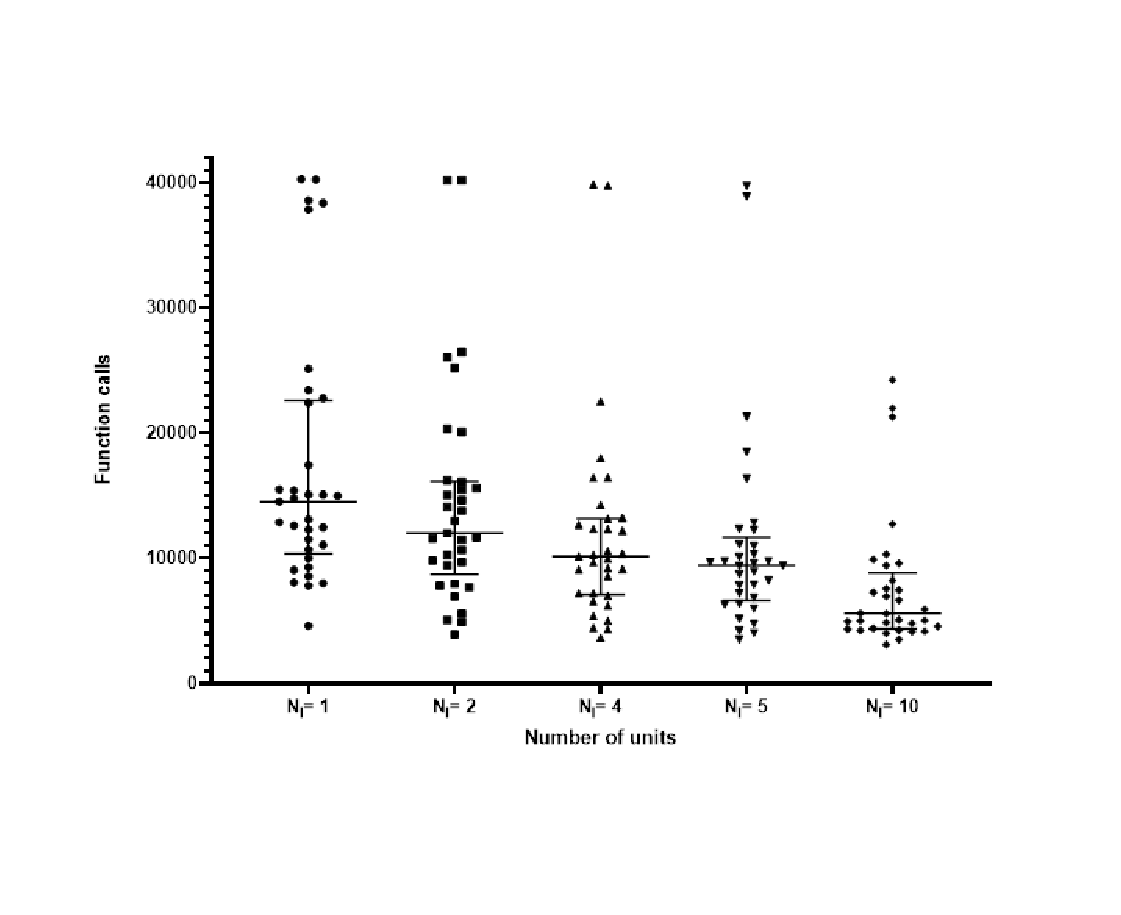
\includegraphics[scale=0.7]{nonparametric}
\par\end{centering}
\caption{We conducted a Friedman test to determine whether there were significant
differences in the scores of function calls on five (N i =1, 2, 4,
5, and 10) repeated number of units. The Friedman chi- square was
94.38 with 4 degrees of freedom, indicating a significant difference
between the groups ($p<0.0001$).\label{fig:nonPar}}

\end{figure}

From the experimental results it is clear that increasing the number
of parallel processing nodes further reduces the total number of function
calls, since more units are used in the attempt to find the global
minimum. In addition, a slight increase in the reliability of the
method in finding the total minimum is also observed.

Furthermore, to determine the effect of the propagation mechanism
on the reliability and speed of the method, another comparative experiment
was performed, in which the number of parallel processing units was
set to 5 ($N_{I}$ = 5) and all propagation mechanisms were used.
The results for this experiment are presented in Table \ref{tab:propagationExperiment}.

\begin{table}[H]
\caption{Comparison of different propagation schemes. The number of processing
units was set to 5.\label{tab:propagationExperiment}}

\raggedright{}%
\begin{tabular}{|c|c|c|c|c|}
\hline 
Function & 1to1 & 1toN & Nto1 & NtoN\tabularnewline
\hline 
\hline 
BF1 & 10315 & 8408 & 9471 & 8647\tabularnewline
\hline 
BF2 & 9403 & 8024 & 10578 & 7730\tabularnewline
\hline 
BRANIN & 5170 & 4633 & 5203 & 5789\tabularnewline
\hline 
CIGAR10 & 38887 & 25035 & 35527 & 34258\tabularnewline
\hline 
CM4 & 12339 & 14195 & 12296 & 12565\tabularnewline
\hline 
DISCUS10 & 10989 & 6484 & 7667 & 6154\tabularnewline
\hline 
EASOM & 3513 & 3072 & 3496 & 3121\tabularnewline
\hline 
ELP10 & 11100 & 13027 & 9598 & 7091\tabularnewline
\hline 
EXP4 & 9556 & 10654 & 9517 & 10607\tabularnewline
\hline 
EXP16 & 21307 & 29289 & 23833 & 27307\tabularnewline
\hline 
EXP64 & 39731 & 11959 & 38191 & 26175\tabularnewline
\hline 
GKLS250 & 6853 & 6568 & 6966 & 7808\tabularnewline
\hline 
GKLS350 & 10095 & 10366 & 10400 & 9674\tabularnewline
\hline 
GRIEWANK2 & 8926 & 6022 & 7791 & 5432\tabularnewline
\hline 
POTENTIAL3 & 4756 & 4011 & 4591 & 4075\tabularnewline
\hline 
POTENTIAL5 & 4221 & 4002 & 4176 & 3870\tabularnewline
\hline 
HANSEN & 4031 & 3092 & 4320 & 3265\tabularnewline
\hline 
HARTMAN3 & 9711 & 10154 & 9316 & 11110\tabularnewline
\hline 
HARTMAN6 & 7194 & 6914(0.73) & 6760(0.97) & 11242(0.73)\tabularnewline
\hline 
RASTRIGIN & 5974 & 4077 & 5383 & 4804\tabularnewline
\hline 
ROSENBROCK4 & 12244 & 13930 & 11511 & 14710\tabularnewline
\hline 
ROSENBROCK8 & 18508 & 15423 & 16659 & 20848\tabularnewline
\hline 
SHEKEL5 & 7898(0.93) & 9604(0.90) & 7513(0.93) & 10657(0.67)\tabularnewline
\hline 
SHEKEL7 & 8717(0.97) & 12204 & 9404 & 10805(0.70)\tabularnewline
\hline 
SHEKEL10 & 8229(0.93) & 13418(0.93) & 9693 & 12677(0.83)\tabularnewline
\hline 
SINU4 & 12842 & 14757 & 13154 & 13376\tabularnewline
\hline 
SINU8 & 16375 & 22754 & 17026 & 20121\tabularnewline
\hline 
TEST2N4 & 9769 & 6633(0.97) & 10289 & 7483(0.83)\tabularnewline
\hline 
TEST2N5 & 9440(0.93) & 4819(0.93) & 8077(0.90) & 5429(0.80)\tabularnewline
\hline 
TEST2N6 & 7855(0.57) & 5358(0.77) & 8354(0.60) & 5574(0.43)\tabularnewline
\hline 
TEST2N7 & 9773(0.50) & 5183(0.33) & 7417(0.53) & 6312(0.40)\tabularnewline
\hline 
TEST30N3 & 6382 & 6538 & 6176 & 7462\tabularnewline
\hline 
TEST30N4 & 6317 & 6938 & 6473 & 6305\tabularnewline
\hline 
\textbf{TOTAL} & \textbf{368460(0.96)} & \textbf{327545(0.96)} & \textbf{356826(0.97)} & \textbf{352483(0.92)}\tabularnewline
\hline 
\end{tabular}
\end{table}
This time, the experimental results did not show any clear superiority
of one of the propagation methods. However, it appears that the 1-to-N
propagation method has slightly better performances than the rest
of the best particle propagation techniques among the sub-populations.

The last experiment had to do with the effect of the $N_{P}$ parameter
on the speed of the method. In it, 5 parallel computing units were
used and the propagation method was set to \textbf{Nto1}. The experimental
results are presented in the Table \ref{tab:npresults}.

\begin{table}[H]
\caption{The effect of the parameter $N_{P}$ to the speed of the proposed
method. The number of threads was set to 5 and the value of $N_{P}$
was changed from 1 to 10.\label{tab:npresults} The propagation scheme
used was Nto1.}

\raggedright{}%
\begin{tabular}{|c|c|c|c|c|c|}
\hline 
Function & $N_{P}=1$ & $N_{P}=2$ & $N_{P}=3$ & $N_{P}=5$ & $N_{P}=10$\tabularnewline
\hline 
\hline 
BF1 & 10114 & 9976 & 10257 & 9471 & 9307\tabularnewline
\hline 
BF2 & 9224 & 10413 & 10051 & 10578 & 9530\tabularnewline
\hline 
BRANIN & 7037 & 6027 & 6238 & 5203 & 4851\tabularnewline
\hline 
CIGAR10 & 39244 & 35793 & 35811 & 35527 & 35835\tabularnewline
\hline 
CM4 & 11839 & 11588 & 12061 & 12296 & 11878\tabularnewline
\hline 
DISCUS10 & 8078 & 6950 & 9671 & 7667 & 11977\tabularnewline
\hline 
EASOM & 3669 & 3538 & 3589 & 3496 & 3477\tabularnewline
\hline 
ELP10 & 11656 & 12382 & 10643 & 9598 & 9641\tabularnewline
\hline 
EXP4 & 9257 & 9340 & 9395 & 9517 & 9626\tabularnewline
\hline 
EXP16 & 27275 & 24008 & 22906 & 23833 & 23190\tabularnewline
\hline 
EXP64 & 39679 & 37334 & 32126 & 38191 & 31119\tabularnewline
\hline 
GKLS250 & 7250 & 6893 & 7116 & 6966 & 6568\tabularnewline
\hline 
GKLS350 & 10281 & 9236 & 10088 & 10400 & 9552\tabularnewline
\hline 
GRIEWANK2 & 9259 & 10096 & 10297 & 7791 & 9527\tabularnewline
\hline 
POTENTIAL3 & 8471 & 6694 & 5770 & 4591 & 4829\tabularnewline
\hline 
POTENTIAL5 & 7127 & 5869 & 5301 & 4176 & 4844\tabularnewline
\hline 
HANSEN & 7978 & 6230 & 5591 & 4320 & 4573\tabularnewline
\hline 
HARTMAN3 & 10162 & 9939 & 10131 & 9316 & 10081\tabularnewline
\hline 
HARTMAN6 & 10614 & 9033 & 8059 & 6760 & 7507\tabularnewline
\hline 
RASTRIGIN & 7491 & 6384 & 6876 & 5383 & 5540\tabularnewline
\hline 
ROSENBROCK4 & 22600 & 16513 & 13631 & 11511 & 12169\tabularnewline
\hline 
ROSENBROCK8 & 34125 & 23004 & 21027 & 16659 & 19740\tabularnewline
\hline 
SHEKEL5 & 12299 & 11923 & 9521 & 7513 & 7256\tabularnewline
\hline 
SHEKEL7 & 13895 & 12358 & 10239 & 9404 & 9471\tabularnewline
\hline 
SHEKEL10 & 14130 & 11536 & 10235 & 9693 & 6936\tabularnewline
\hline 
SINU4 & 12760 & 12601 & 12268 & 13154 & 11905\tabularnewline
\hline 
SINU8 & 16957 & 17327 & 16346 & 17026 & 17030\tabularnewline
\hline 
TEST2N4 & 12215 & 9152 & 8136 & 10289 & 10024\tabularnewline
\hline 
TEST2N5 & 11384 & 8429 & 7934 & 8077 & 8935\tabularnewline
\hline 
TEST2N6 & 11833 & 8101 & 7825 & 8354 & 9655\tabularnewline
\hline 
TEST2N7 & 11162 & 8362 & 8692 & 7417 & 9486\tabularnewline
\hline 
TEST30N3 & 7178 & 7015 & 6829 & 6176 & 6216\tabularnewline
\hline 
TEST30N4 & 6518 & 6676 & 6509 & 6473 & 6756\tabularnewline
\hline 
\textbf{TOTAL} & \textbf{442761} & \textbf{390720} & \textbf{371169} & \textbf{356826} & \textbf{359031}\tabularnewline
\hline 
\end{tabular}
\end{table}
As is evident, increasing the value of the $N_{P}$ parameter significantly
reduces the required number of function calls up to a value of 5.
From then on, the total number of calls appears to be constant. Practically,
this means that sending not only the best particle but also those
with the immediately lower value further reduces the required number
of function calls.

\subsection{Experiments for the execution time }

To understand the efficiency of the method with respect to execution
time, three additional series of experiments were performed. In all
experiments, the total number of particles in the particle swarm optimization
was fixed at 500 and from 1 to 20 parallel processing units were used
and the total execution time was measured for 30 different independent
runs. The experiments were conducted on AMD Epyc 7552 equipped with
32GB of RAM. The operating system was the Ubuntu 20.04 operating system.

During the first series of the additional experiments, the High Conditioned
Elliptic function, defined as 
\[
f(x)=\sum_{i=1}^{n}\left(10^{6}\right)^{\frac{i-1}{n-1}}x_{i}^{2}
\]
was used as a test case. In the experiments, the values n=10,20,30,40,50
were used and the experimental results are displayed graphically in
the figure \ref{fig:elpTime}. 

\begin{figure}[H]
\begin{centering}
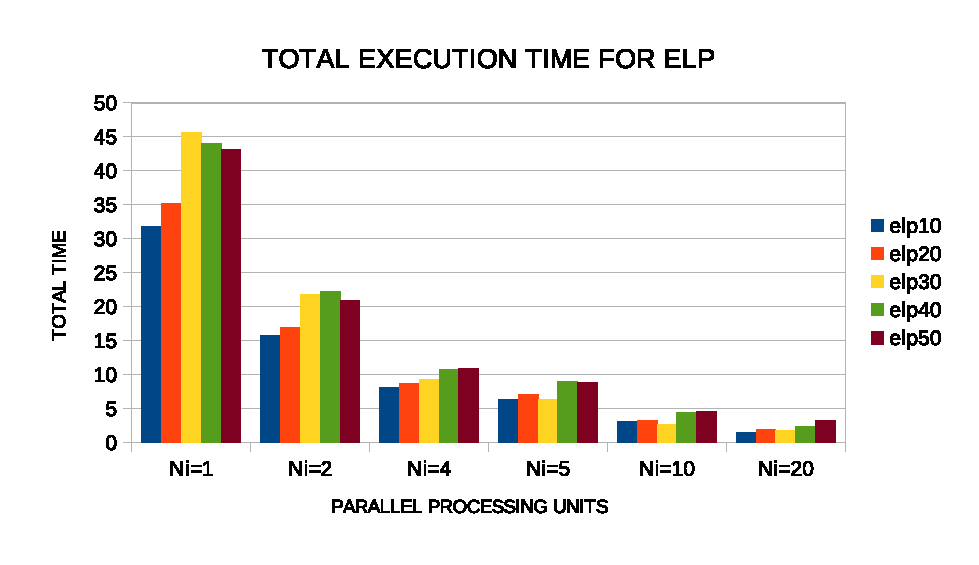
\includegraphics[scale=0.7]{elp_time}
\par\end{centering}
\caption{Total execution time for different number of parallel processing threads
for the objective function ELP.\label{fig:elpTime}}

\end{figure}
From the experimental results, it follows that doubling the parallel
processing units almost halves the required execution time in most
cases.

During the second series of experiments, different versions of the
GKLS function were used for dimensions from 2 to 5. This function
was thoroughly tested also in the work of Sergeyev et al \citep{Sergeyev}.
In each dimension, 10 different instances of the function were used
to have a safe estimate of both the performance of the method and
the possible decrease in execution time as the parallel processing
units.\textbf{ }The average execution time for different dimensions
of the GKLS function and for different numbers of processing units
is graphically shown in Figure \ref{fig:gklsTime}. 
\begin{figure}[H]
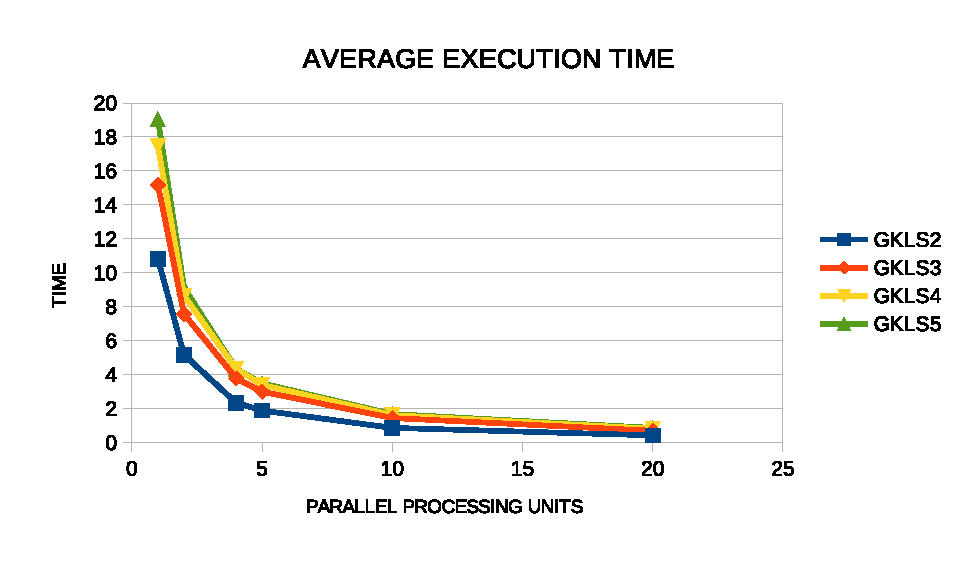
\includegraphics[scale=0.8]{gklstime}

\caption{Average time execution for the GKLS function. The dimension of the
function varies from 2 to 5.\label{fig:gklsTime}}

\end{figure}
As is shown, the execution time decreases rapidly with increasing
parallel processing units in all instances of the function. Furthermore,
the average number of function calls for every case is also measured
and the results are plotted in Figure \ref{fig:gklsCalls}. 
\begin{figure}[H]
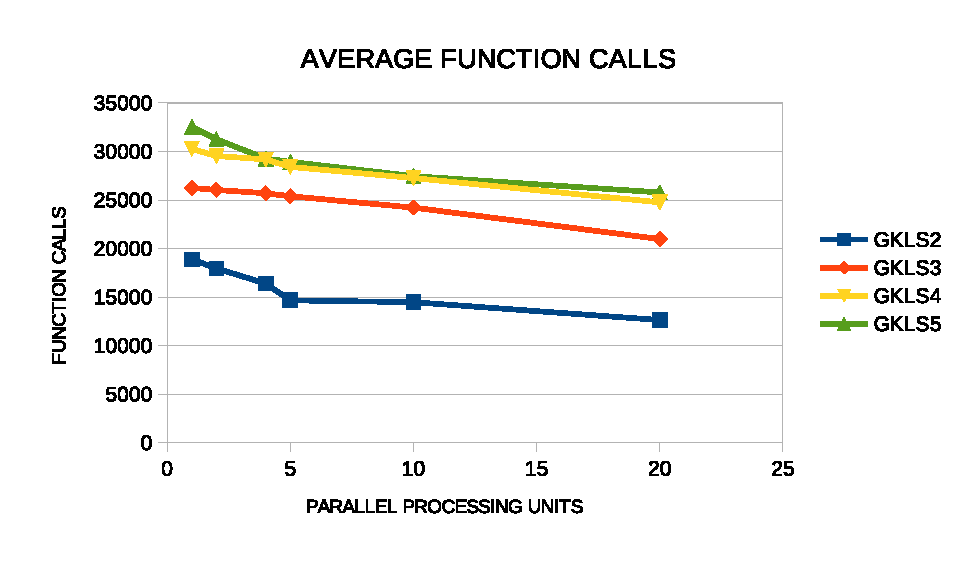
\includegraphics[scale=0.8]{gklscalls}

\caption{Average function calls for different cases of the GKLS function. \label{fig:gklsCalls}}

\end{figure}
Increasing the number of parallel processing units also reduces the
number of required function calls, especially for the low-dimensional
cases (Gkls2 and Gkls3). However, the most interesting point of this
series of experiments is the ability of the proposed technique to
locate the global minimum as the number of parallel computing units
increases. This capability is graphically represented in Figure \ref{fig:gklsRate}.
\begin{figure}[H]
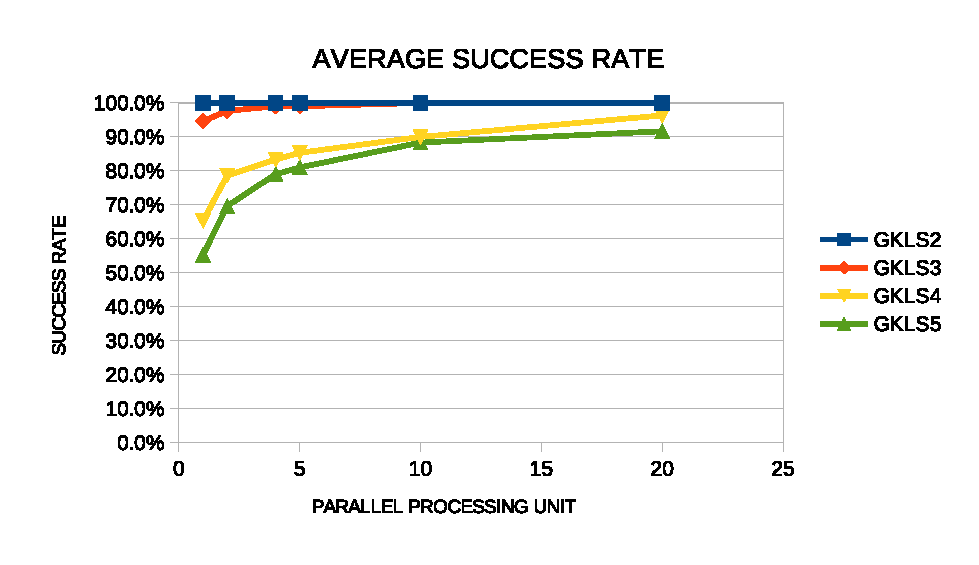
\includegraphics[scale=0.8]{gklsrate}

\caption{Average success rate in finding the global minimum for different cases
of the Gkls function.\label{fig:gklsRate}}

\end{figure}
 From this graph it can be concluded that the increase in parallel
processing units significantly improves the efficiency of the technique
in finding the global minimum.

In the third series of additional experiments, a more difficult experiment
was used, but one that has multiple applications. The proposed method
was used to train an artificial neural network \citep{nn1,nn2} with
10 processing nodes applied on two widely used classification problems
from the relevant literature: the Wine problem \citep{wine1,wine2}
and the Parkinsons problem \citep{parkinsons}.

\begin{figure}[H]
\begin{centering}
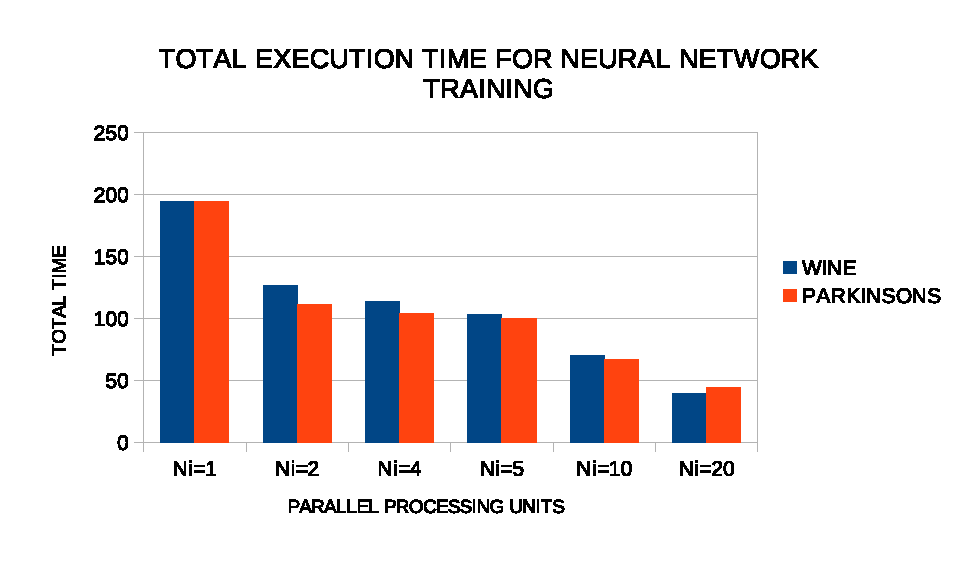
\includegraphics[scale=0.8]{mlp_time.eps}
\par\end{centering}
\caption{Total execution time for different number of parallel processing threads
for neural network training for two classification datasets\label{fig:mlpTime}}

\end{figure}
Again, the required training time decreases drastically with increasing
parallel processing units.

\section{Conclusions\label{sec:Conclusions}}

In the present work a number of ideas were presented that can lead
to an efficient parallel implementation of the PSO technique. The
need for parallelization of the method is great, as it is an iterative
process involving repeated operations on vectors and these operations
for large problems may require significantly large computational time.
In the current work, a technique of propagating the best particles
between computing units as well as a termination rule of the overall
process were introduced. In the case of the propagation of the best
particles from the experiments carried out, it appears that it is
more efficient to send between the computing units more than the best
particle. Furthermore, the propagation method between parallel computing
units did not have a drastic effect on the efficiency and speed of
the method, although the 1-to-N propagation method appeared to have
slightly better results. Furthermore, the increase of the parameter
$N_{P}$ from 1 to 5 decreased the required number of function calls.
However, the biggest gain from using the method lies in the increase
in parallel processing units. From the experiments performed, it is
evident that as parallel processing units increase, the total function
calls required to find the global minimum decreases almost for every
objective function. In addition, the increase in parallel processing
units improved to some extent the efficiency of the method in finding
the global minimum. The effectiveness of the proposed method was also
shown in the comparison between its serial version and two other widely
available techniques in the relevant literature. In this comparison
the serial version of the method required significantly fewer function
calls to find each global minimum.

On a percentage basis, the proposed technique significantly outperforms
the other two compared global optimization techniques. The serial
version of the proposed technique reduces the required number of function
calls by 22\%-28\% compared to the genetic algorithm and the particle
swarm optimization techniques respectively. However, with the use
of more processing units, the reduction in the number of function
calls reaches approximately 70\%. Furthermore, from the relevant experiments
done on the actual execution time, it appears that any doubling of
parallel processing threads halves the required execution time required
to find the global minimum.

In the future, the important work done in the parallelization of the
PSO technique can be continued with the use of new termination rules
that will be suitable for execution in parallel computing environments
but also a possible extension of the best particle propagation techniques
between parallel computing units.

\vspace{6pt}


\authorcontributions{I.G.T. and V.C. conceived of the idea, the methodology and they have
implemented the corresponding software. I.G.T. conducted the experiments,
employing objective functions as test cases, and provided the comparative
experiments. V.C. performed the statistical analysis and prepared
the manuscript. All authors have read and agreed to the published
version of the manuscript.}

\funding{This research received no external funding.}

\institutionalreview{Not applicable.}

\informedconsent{Not applicable. }

\institutionalreview{Not applicable.}

\acknowledgments{The experiments of this research work were performed at the high
performance computing system established at Knowledge and Intelligent
Computing Laboratory, Department of Informatics and Telecommunications,
University of Ioannina, acquired with the project “Educational Laboratory
equipment of TEI of Epirus” with MIS 5007094 funded by the Operational
Programme “Epirus” 2014--2020, by ERDF and national funds.}

\conflictsofinterest{The authors declare no conflict of interest.}

\sampleavailability{Not applicable.}

\appendixtitles{}

\appendixstart{}

\appendix

\begin{adjustwidth}{-\extralength}{0cm}{}

\reftitle{References}
\begin{thebibliography}{999}
\bibitem{go_physics1}L. Yang, D. Robin, F. Sannibale, C. Steier,
W. Wan, Global optimization of an accelerator lattice using multiobjective
genetic algorithms, Nuclear Instruments and Methods in Physics Research
Section A: Accelerators, Spectrometers, Detectors and Associated Equipment
\textbf{609}, pp. 50-57, 2009.

\bibitem{go_physics2}E. Iuliano, Global optimization of benchmark
aerodynamic cases using physics-based surrogate models, Aerospace
Science and Technology \textbf{67}, pp.273-286, 2017.

\bibitem{go_physics3}Q. Duan, S. Sorooshian, V. Gupta, Effective
and efficient global optimization for conceptual rainfall-runoff models,
Water Resources Research \textbf{28}, pp. 1015-1031 , 1992.

\bibitem{go_chem1}S. Heiles, R. L. Johnston, Global optimization
of clusters using electronic structure methods, Int. J. Quantum Chem.
\textbf{113}, pp. 2091-- 2109, 2013.

\bibitem{go_chem2}W.H. Shin, J.K. Kim, D.S. Kim, C. Seok, GalaxyDock2:
Protein--ligand docking using beta-complex and global optimization,
J. Comput. Chem. \textbf{34}, pp. 2647-- 2656, 2013.

\bibitem{go_chem3}A. Liwo, J. Lee, D.R. Ripoll, J. Pillardy, H. A.
Scheraga, Protein structure prediction by global optimization of a
potential energy function, Biophysics \textbf{96}, pp. 5482-5485,
1999.

\bibitem{go_econ1}Zwe-Lee Gaing, Particle swarm optimization to solving
the economic dispatch considering the generator constraints, IEEE
Transactions on \textbf{18} Power Systems, pp. 1187-1195, 2003.

\bibitem{go_econ2}C. D. Maranas, I. P. Androulakis, C. A. Floudas,
A. J. Berger, J. M. Mulvey, Solving long-term financial planning problems
via global optimization, Journal of Economic Dynamics and Control
\textbf{21}, pp. 1405-1425, 1997.

\bibitem{go_med1}Eva K. Lee, Large-Scale Optimization-Based Classification
Models in Medicine and Biology, Annals of Biomedical Engineering \textbf{35},
pp 1095-1109, 2007.

\bibitem{go_med2}Y. Cherruault, Global optimization in biology and
medicine, Mathematical and Computer Modelling \textbf{20}, pp. 119-132,
1994.

\bibitem{interval1}M.A. Wolfe, Interval methods for global optimization,
Applied Mathematics and Computation \textbf{75}, pp. 179-206, 1996.

\bibitem{interval2}T. Csendes and D. Ratz, Subdivision Direction
Selection in Interval Methods for Global Optimization, SIAM J. Numer.
Anal. \textbf{34}, pp. 922--938, 1997. 

\bibitem{determ1}C.D Maranas, C.A. Floudas, A deterministic global
optimization approach for molecular structure determination, J. Chem.
Phys. \textbf{100}, 1247, 1994.

\bibitem{determ2}J. Barhen, V. Protopopescu, D. Reister, TRUST: A
Deterministic Algorithm for Global Optimization, Science \textbf{276},
pp. 1094-1097, 1997.

\bibitem{determ3}Y. Evtushenko, M.A. Posypkin, deterministic approach
to global box-constrained optimization, Optim Lett \textbf{7}, pp.
819--829, 2013.

\bibitem{determ4}Y.D. Sergeyev, D.E. Kvasov, A deterministic global
optimization using smooth diagonal auxiliary functions, Communications
in Nonlinear Science and Numerical Simulation \textbf{21}, pp. 99-111,
2015.

\bibitem{determ5}C. Kunde, D. Michaels, J. Micovic, P. Lutze, A.
Górak, A. Kienle, Deterministic global optimization in conceptual
process design of distillation and melt crystallization, Chemical
Engineering and Processing: Process Intensification \textbf{99}, pp.
132-142, 2016.

\bibitem{Sergeyev}Y.D. Sergeyev, D.E. Kvasov, M.S. Mukhametzhanov,
On the efficiency of nature-inspired metaheuristics in expensive global
optimization with limited budget. Sci Rep \textbf{8}, 453, 2018.

\bibitem{crs1}W. L. Price, Global optimization by controlled random
search, Journal of Optimization Theory and Applications \textbf{40},
pp. 333-348, 1983.

\bibitem{crs2}Ivan Křivý, Josef Tvrdík, The controlled random search
algorithm in optimizing regression models, Computational Statistics
\& Data Analysis \textbf{20}, pp. 229-234, 1995.

\bibitem{crs3}M.M. Ali, A. Törn, and S. Viitanen, A Numerical Comparison
of Some Modified Controlled Random Search Algorithms, Journal of Global
Optimization \textbf{11},pp. 377--385,1997.

\bibitem{simann_major}S. Kirkpatrick, CD Gelatt, , MP Vecchi, Optimization
by simulated annealing, Science \textbf{220}, pp. 671-680, 1983.

\bibitem{simann1}L. Ingber, Very fast simulated re-annealing, Mathematical
and Computer Modelling \textbf{12}, pp. 967-973, 1989.

\bibitem{simann2}R.W. Eglese, Simulated annealing: A tool for operational
research, Simulated annealing: A tool for operational research \textbf{46},
pp. 271-281, 1990.

\bibitem{diffe1}R. Storn, K. Price, Differential Evolution - A Simple
and Efficient Heuristic for Global Optimization over Continuous Spaces,
Journal of Global Optimization \textbf{11}, pp. 341-359, 1997.

\bibitem{diffe2}J. Liu, J. Lampinen, A Fuzzy Adaptive Differential
Evolution Algorithm. Soft Comput \textbf{9}, pp.448--462, 2005.

\bibitem{pso_major}J. Kennedy and R. Eberhart, \textquotedbl Particle
swarm optimization,\textquotedbl{} Proceedings of ICNN'95 - International
Conference on Neural Networks, 1995, pp. 1942-1948 vol.4, doi: 10.1109/ICNN.1995.488968.

\bibitem{pso1}Riccardo Poli, James Kennedy kennedy, Tim Blackwell,
Particle swarm optimization An Overview, Swarm Intelligence \textbf{1},
pp 33-57, 2007. 

\bibitem{pso2}Ioan Cristian Trelea, The particle swarm optimization
algorithm: convergence analysis and parameter selection, Information
Processing Letters \textbf{85}, pp. 317-325, 2003.

\bibitem{aco1}M. Dorigo, M. Birattari and T. Stutzle, Ant colony
optimization, IEEE Computational Intelligence Magazine \textbf{1},
pp. 28-39, 2006.

\bibitem{aco2}K. Socha, M. Dorigo, Ant colony optimization for continuous
domains, European Journal of Operational Research 185, pp. 1155-1173,
2008.

\bibitem{ga1}D. Goldberg, Genetic Algorithms in Search, Optimization
and Machine Learning, Addison-Wesley Publishing Company, Reading,
Massachussets, 1989.

\bibitem{ga2}Z. Michaelewicz, Genetic Algorithms + Data Structures
= Evolution Programs. Springer - Verlag, Berlin, 1996.

\bibitem{ga3}S.A. Grady, M.Y. Hussaini, M.M. Abdullah, Placement
of wind turbines using genetic algorithms, Renewable Energy \textbf{30},
pp. 259-270, 2005.

\bibitem{gpu1}Y. Zhou and Y. Tan, \textquotedbl GPU-based parallel
particle swarm optimization,\textquotedbl{} 2009 IEEE Congress on
Evolutionary Computation, pp. 1493-1500, 2009.

\bibitem{gpu2}L. Dawson and I. Stewart, \textquotedbl Improving
Ant Colony Optimization performance on the GPU using CUDA,\textquotedbl{}
2013 IEEE Congress on Evolutionary Computation, 2013, pp. 1901-1908,
doi: 10.1109/CEC.2013.6557791.

\bibitem{gpu3}Barkalov, K., Gergel, V. Parallel global optimization
on GPU. J Glob Optim 66, 3--20 (2016). 

\bibitem{meta1}I. BoussaïD, J. Lepagnot, P. Siarry, P., A survey
on optimization metaheuristics. Information sciences \textbf{237},
pp. 82-117, 2013.

\bibitem{meta2}T. Dokeroglu, E. Sevinc, T. Kucukyilmaz, A. Cosar,
A survey on new generation metaheuristic algorithms. Computers \&
Industrial Engineering \textbf{137}, 106040, 2019.

\bibitem{meta3}K. Hussain, M.N.M. Salleh, S. Cheng, Y. Shi, Metaheuristic
research: a comprehensive survey.Artificial Intelligence Review \textbf{52},
pp. 2191-2233, 2019.

\bibitem{psophysics1}Anderson Alvarenga de Moura Meneses, Marcelo
Dornellas, Machado Roberto Schirru, Particle Swarm Optimization applied
to the nuclear reload problem of a Pressurized Water Reactor, Progress
in Nuclear Energy \textbf{51}, pp. 319-326, 2009.

\bibitem{psophysics2}Ranjit Shaw, Shalivahan Srivastava, Particle
swarm optimization: A new tool to invert geophysical data, Geophysics
\textbf{72}, 2007.

\bibitem{psochem1}C. O. Ourique, E.C. Biscaia, J.C. Pinto, The use
of particle swarm optimization for dynamical analysis in chemical
processes, Computers \& Chemical Engineering \textbf{26}, pp. 1783-1793,
2002.

\bibitem{psochem2}H. Fang, J. Zhou, Z. Wang et al, Hybrid method
integrating machine learning and particle swarm optimization for smart
chemical process operations, Front. Chem. Sci. Eng. \textbf{16}, pp.
274--287, 2022.

\bibitem{psomed1}M.P. Wachowiak, R. Smolikova, Yufeng Zheng, J.M.
Zurada, A.S. Elmaghraby, An approach to multimodal biomedical image
registration utilizing particle swarm optimization, IEEE Transactions
on Evolutionary Computation \textbf{8}, pp. 289-301, 2004.

\bibitem{psomed2}Yannis Marinakis. Magdalene Marinaki, Georgios Dounias,
Particle swarm optimization for pap-smear diagnosis, Expert Systems
with Applications \textbf{35}, pp. 1645-1656, 2008. 

\bibitem{psoecon}Jong-Bae Park, Yun-Won Jeong, Joong-Rin Shin, Kwang
Y. Lee, An Improved Particle Swarm Optimization for Nonconvex Economic
Dispatch Problems, IEEE Transactions on Power Systems \textbf{25},
pp. 156-16\textbf{216}6, 2010.

\bibitem{psoApp1}B. Liu, L. Wang, Y.H. Jin, An Effective PSO-Based
Memetic Algorithm for Flow Shop Scheduling, IEEE Transactions on Systems,
Man, and Cybernetics, Part B (Cybernetics) \textbf{37}, pp. 18-27,
2007.

\bibitem{psoApp2}J. Yang, L. He, S. Fu, An improved PSO-based charging
strategy of electric vehicles in electrical distribution grid, Applied
Energy \textbf{128}, pp. 82-92, 2014.

\bibitem{psoApp3}K. Mistry, L. Zhang, S. C. Neoh, C. P. Lim, B. Fielding,
A Micro-GA Embedded PSO Feature Selection Approach to Intelligent
Facial Emotion Recognition, IEEE Transactions on Cybernetics. \textbf{47},
pp. 1496-1509, 2017.

\bibitem{psoApp4}S. Han, X. Shan, J. Fu, W. Xu, H. Mi, Industrial
robot trajectory planning based on improved pso algorithm, J. Phys.:
Conf. Ser. \textbf{1820}, 012185, 2021.

\bibitem{psoReview}F. Marini, B. Walczak, Particle swarm optimization
(PSO). A tutorial, Chemometrics and Intelligent Laboratory Systems
\textbf{149}, pp. 153-165, 2015.

\bibitem{psoOverview}M. Jain, V. Saihjpal, N. Singh, S.B. Singh,
An Overview of Variants and Advancements of PSO Algorithm, Applied
Sciences \textbf{12}, 8392, 2022. 

\bibitem{pso_mutation1}A. Stacey, M. Jancic, I. Grundy, Particle
swarm optimization with mutation, In: 2003 Congress on Evolutionary
Computation, 2003. CEC '03., pp. 1425-1430, 2003.

\bibitem{pso_mutation2}M. Pant, R. Thangaraj, A. Abraham, Particle
Swarm Optimization Using Adaptive Mutation, In: 2008 19th International
Workshop on Database and Expert Systems Applications, pp. 519-523,
2008.

\bibitem{pso_mutation3}N. Higashi, H. Iba, Particle swarm optimization
with Gaussian mutation, In: Proceedings of the 2003 IEEE Swarm Intelligence
Symposium. SIS'03 (Cat. No.03EX706), pp. 72-79, 2003.

\bibitem{pso_initvelocity}A. Engelbrecht, \textquotedbl Particle
swarm optimization: Velocity initialization,\textquotedbl{} 2012 IEEE
Congress on Evolutionary Computation, pp. 1-8, 2012.

\bibitem{psohybrid1}B. Liu, L. Wang, Y.H. Jin, F. Tang, D.X. Huang,
Improved particle swarm optimization combined with chaos, Chaos Solitons
and Fractals \textbf{25}, pp. 1261-1271, 2005.

\bibitem{psohybrid2}X.H. Shi, Y.C. Liang, H.P. Lee, C. Lu, L.M. Wang,
An improved GA and a novel PSO-GA based hybrid algorithm, Information
Processing Letters \textbf{93}, pp. 255-261, 2005.

\bibitem{psohybrid3}Harish Garg, A hybrid PSO-GA algorithm for constrained
optimization problems, Applied Mathematics and Computation \textbf{274},
pp. 292-305, 2016.

\bibitem{pso_parallel1}J. F. Schutte, J. A. Reinbolt, B. J. Fregly,
R. T. Haftka, A. D. George, Parallel global optimization with the
particle swarm algorithm, Int. J. Numer. Meth. Engng. \textbf{61},
pp. 2296-2315, 2004.

\bibitem{pso_parallel2}B-Il Koh, A.D. George, R.T. Haftka, B.J. Fregly,
Parallel asynchronous particle swarm optimization. Int. J. Numer.
Meth. Engng., \textbf{67}, pp. 578-595, 2006.

\bibitem{pso_parallel3}G. Venter, J. Sobieszczanski-Sobieski, Parallel
Particle Swarm Optimization Algorithm Accelerated by Asynchronous
Evaluations, Journal of Aerospace Computing, Information, and Communication
\textbf{3}, pp. 123-137, 2006.

\bibitem{pso_velocity1}Z.L. Gaing, Particle swarm optimization to
solving the economic dispatch considering the generator constraints,
IEEE Transactions on Power Systems \textbf{18}, pp. 1187-1195, 2003.

\bibitem{pso_velocity2}X. Yang, Jinsha Yuan, Jiangy Yuan, H. Mao,
A modified particle swarm optimizer with dynamic adaptation, Applied
Mathematics and Computation \textbf{189}, pp. 1205-1213, 2007.

\bibitem{pso_velocity3}Y. Jiang, T. Hu, C. Huang, X. Wu, An improved
particle swarm optimization algorithm, Applied Mathematics and Computation
\textbf{193}, pp. 231-239, 2007.

\bibitem{ge_pso1}A. Bogdanova, J.P. Junior, C. Aranha, Franken-Swarm:
Grammatical Evolution for the Automatic Generation of Swarm-like Meta-Heuristics,
In: Proceedings of the Genetic and Evolutionary Computation Conference
Companion, pp. 411-412, 2019.

\bibitem{ge_mainpaper}M. O'Neill, C. Ryan, Grammatical evolution,IEEE
Transactions on Evolutionary Computation \textbf{5}, pp. 349-358,
2001.

\bibitem{siman_pso}X. Pan, L. Xue, Y. Lu et al, Hybrid particle swarm
optimization with simulated annealing, Multimed Tools Appl \textbf{78},
pp. 29921--29936, 2019.

\bibitem{simman_pso_energy}M.A. Mughal, Q. Ma, C. Xiao, Photovoltaic
Cell Parameter Estimation Using Hybrid Particle Swarm Optimization
and Simulated Annealing, Energies \textbf{10}, 2017.

\bibitem{pso_de}G.H. Lin, J. Zhang, Z.H. Liu, Hybrid particle swarm
optimization with differential evolution for numerical and engineering
optimization. Int. J. Autom. Comput. \textbf{15}, pp. 103--114, 2018.

\bibitem{pso_local1}S. Li, M. Tan, I. W. Tsang, J. T. -Y. Kwok, A
Hybrid PSO-BFGS Strategy for Global Optimization of Multimodal Functions,
IEEE Transactions on Systems, Man, and Cybernetics, Part B (Cybernetics)
\textbf{41}, pp. 1003-1014, 2011.

\bibitem{pso_local2}G. Wu, D. Qiu, Y. Yu, W. Pedrycz, M. Ma, H. Li,
Superior solution guided particle swarm optimization combined with
local search techniques, Expert Systems with Applications \textbf{41},
pp. 7536-7548, 2014.

\bibitem{parallel_go1}J. Olenšek, T. Tuma, J. Puhan, Á Bűrmen, A
new asynchronous parallel global optimization method based on simulated
annealing and differential evolution, Applied Soft Computing \textbf{11},
pp. 1481-1489, 2011.

\bibitem{paralleGo2}R.G. Regis, C.A. Shoemaker., Parallel stochastic
global optimization using radial basis functions, INFORMS Journal
on Computing \textbf{21}, pp. 411-426, 2009.

\bibitem{rbf1}J. Park and I. W. Sandberg, Universal Approximation
Using Radial-Basis-Function Networks, Neural Computation \textbf{3},
pp. 246-257, 1991.

\bibitem{parallelReview1}E. Alba, G. Luque, S. Nesmachnow, Parallel
metaheuristics: recent advances and new trends. International Transactions
in Operational Research \textbf{20}, pp. 1-4, 2013.

\bibitem{parallelReview2}M. Essaid, L. Idoumghar, J. Lepagnot, M.
Brévilliers, GPU parallelization strategies for metaheuristics: a
survey. International Journal of Parallel, Emergent and Distributed
Systems \textbf{34}, pp. 497-522, 2019.

\bibitem{ppso1}B.I. Koh, A.D. George, R.T. Haftka, B.J. Fregly, Parallel
asynchronous particle swarm optimization. Int. J. Numer. Meth. Engng.
\textbf{67}, pp. 578-595, 2006.

\bibitem{ppso2}G. S. Tewolde, D. M. Hanna, R. E. Haskell, Multi-swarm
parallel PSO: Hardware implementation, In: 2009 IEEE Swarm Intelligence
Symposium, Nashville, TN, USA, 2009, pp. 60-66, 2009.

\bibitem{ppso3}A. Ouyang, Z. Tang, X. Zhou, Y. Xu, G. Pan, K. Li,
Parallel hybrid PSO with CUDA for lD heat conduction equation, Computers
\& Fluids \textbf{110}, pp. 198-210, 2015.

\bibitem{ppso4}A. de Campos, A.T.R. Pozo, E.P. Duarte, Parallel multi-swarm
PSO strategies for solving many objective optimization problems, Journal
of Parallel and Distributed Computing \textbf{126}, pp. 13-33, 2019.

\bibitem{parallelPsoReview}S. Lalwani, H. Sharma, S.C. Satapathy,
K. Deep, J.C. Bansal, A survey on parallel particle swarm optimization
algorithms. Arabian Journal for Science and Engineering \textbf{44},
pp. 2899-2923, 2019.

\bibitem{RandomInertia}R.C. Eberhart, Y.H. Shi, Tracking and optimizing
dynamic systems with particle swarms, in: Congress on Evolutionary
Computation, Korea, 2001.

\bibitem{ipso}V. Charilogis, I.G. Tsoulos, Toward an Ideal Particle
Swarm Optimizer for Multidimensional Functions, Information \textbf{13},
217, 2022.

\bibitem{Powell}M.J.D Powell, A Tolerant Algorithm for Linearly Constrained
Optimization Calculations, Mathematical Programming \textbf{45}, pp.
547-566, 1989. 

\bibitem{Ali1}M. Montaz Ali, Charoenchai Khompatraporn, Zelda B.
Zabinsky, A Numerical Evaluation of Several Stochastic Algorithms
on Selected Continuous Global Optimization Test Problems, Journal
of Global Optimization \textbf{31}, pp 635-672, 2005. 

\bibitem{Floudas1}C.A. Floudas, P.M. Pardalos, C. Adjiman, W. Esposoto,
Z. G$\ddot{\mbox{u}}$m$\ddot{\mbox{u}}$s, S. Harding, J. Klepeis,
C. Meyer, C. Schweiger, Handbook of Test Problems in Local and Global
Optimization, Kluwer Academic Publishers, Dordrecht, 1999.

\bibitem{testfunctions1}M.M. Ali and P. Kaelo, Improved particle
swarm algorithms for global optimization, Applied Mathematics and
Computation \textbf{196}, pp. 578-593, 2008.

\bibitem{testfunctions2}H. Koyuncu, R. Ceylan, A PSO based approach:
Scout particle swarm algorithm for continuous global optimization
problems, Journal of Computational Design and Engineering \textbf{6},
pp. 129--142, 2019.

\bibitem{testfunctions3}Patrick Siarry, Gérard Berthiau, François
Durdin, Jacques Haussy, ACM Transactions on Mathematical Software
\textbf{23}, pp 209--228, 1997.

\bibitem{testfunctions4}I.G. Tsoulos, I.E. Lagaris, GenMin: An enhanced
genetic algorithm for global optimization, Computer Physics Communications\textbf{
178, }pp. 843-851, 2008.

\bibitem{gkls}M. Gaviano, D.E. Ksasov, D. Lera, Y.D. Sergeyev, Software
for generation of classes of test functions with known local and global
minima for global optimization, ACM Trans. Math. Softw. \textbf{29},
pp. 469-480, 2003.

\bibitem{Jones}J.E. Lennard-Jones, On the Determination of Molecular
Fields, Proc. R. Soc. Lond. A \textbf{ 106}, pp. 463--477, 1924.

\bibitem{openmp}R. Chandra, L. Dagum, D. Kohr, D. Maydan,J. McDonald
and R. Menon, Parallel Programming in OpenMP, Morgan Kaufmann Publishers
Inc., 2001.

\bibitem{nn1}C. Bishop, Neural Networks for Pattern Recognition,
Oxford University Press, 1995.

\bibitem{nn2}G. Cybenko, Approximation by superpositions of a sigmoidal
function, Mathematics of Control Signals and Systems \textbf{2}, pp.
303-314, 1989.

\bibitem{wine1}M. Raymer, T.E. Doom, L.A. Kuhn, W.F. Punch, Knowledge
discovery in medical and biological datasets using a hybrid Bayes
classifier/evolutionary algorithm. IEEE transactions on systems, man,
and cybernetics. Part B, Cybernetics : a publication of the IEEE Systems,
Man, and Cybernetics Society, \textbf{33} , pp. 802-813, 2003.

\bibitem{wine2}P. Zhong, M. Fukushima, Regularized nonsmooth Newton
method for multi-class support vector machines, Optimization Methods
and Software \textbf{22}, pp. 225-236, 2007.

\bibitem{parkinsons}M.A. Little, P.E. McSharry, E.J. Hunter, J. Spielman,
L.O. Ramig, Suitability of dysphonia measurements for telemonitoring
of Parkinson's disease. IEEE Trans Biomed Eng. \textbf{56}, pp. 1015-1022,
2009.

\end{thebibliography}

\end{adjustwidth}{}
\end{document}
